%(BEGIN_QUESTION)
% Copyright 2006, Tony R. Kuphaldt, released under the Creative Commons Attribution License (v 1.0)
% This means you may do almost anything with this work of mine, so long as you give me proper credit

Gitt disse to koblingsalternativene (transmitter nær prosess versus langt unna): hvilket er best, og hvorfor?

$$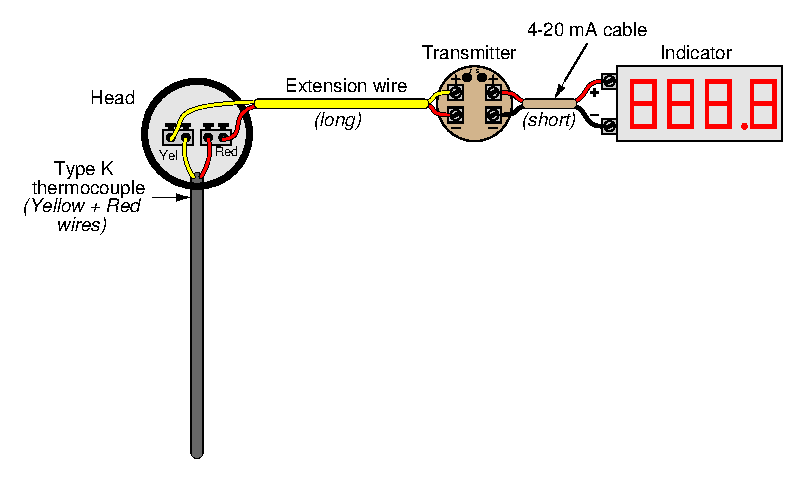
\includegraphics[width=15.5cm]{i00392x01.eps}$$

$$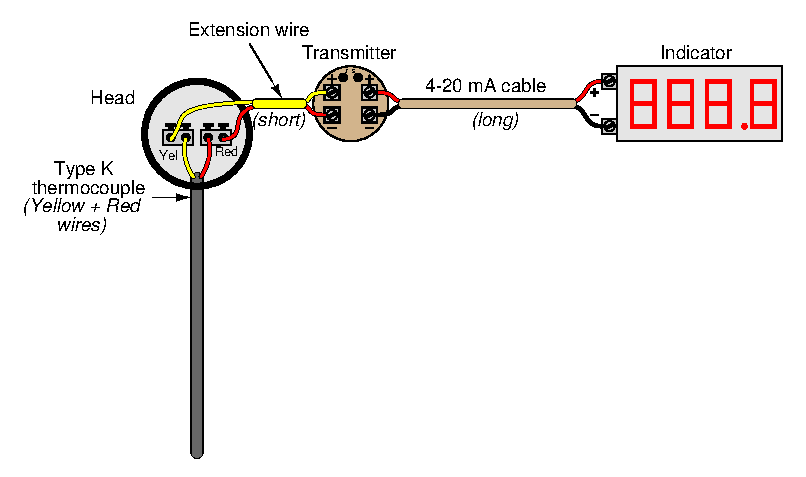
\includegraphics[width=15.5cm]{i00392x02.eps}$$

\vskip 20pt \vbox{\hrule \hbox{\strut \vrule{} {\bf Forslag til sokratisk diskusjon} \vrule} \hrule}

\begin{itemize}
\item{} Hvis den lange kabelen i hvert tilfelle var {\it skjermet}, hvordan bør skjermen jordes for best resultat?
\item{} Hvordan kan vi bruke en {\it loop-kalibrator} for å ``lure'' indikatoren til å tro at termoelementet har en gitt temperatur når det i virkeligheten ikke har det?
\end{itemize}

\underbar{file i00392}
%(END_QUESTION)





%(BEGIN_ANSWER)

Termoelementsignaler er svært små, og inngangsimpedansen i en termoelementtransmitter er vanligvis høy, noe som gjør kretsen utsatt for elektrisk støy. Derfor er det best å minimere lengden på støyutsatt signalvei (termoelementledningen). I tillegg er termoelementledning (selv forlengelseskvalitet) dyrere enn tilsvarende kobber, slik at lange kobberstrekk ofte er rimeligere enn lange termoelementstrekk.

%(END_ANSWER)





%(BEGIN_NOTES)








\vskip 20pt \vbox{\hrule \hbox{\strut \vrule{} {\bf Virtuell feilsøking} \vrule} \hrule}

Denne oppgaven egner seg godt for ``virtuell feilsøking''. Vis diagrammet for studentene og velg i hodet ditt en bestemt feil. Presenter så ett eller flere symptomer (noe en operatør kan observere). Studentene foreslår diagnostiske tester for å finne feiltype og feilplassering, som om de var teknikere i felt. Din rolle er å oppgi testresultater for hvert forslag, synlig for alle studenter.

Under og etter øvelsen er det nyttig å stille oppfølgingsspørsmål som:

\begin{itemize}
\item{} Hva forteller resultatet av siste test om feilen?
\item{} Hvis resultatet hadde vært annerledes, hva ville det fortalt?
\item{} Er siste test den beste vi kan gjøre?
\item{} Hva er ideell testrekkefølge for å finne feilen i færrest mulig steg?
\end{itemize}

%INDEX% Measurement, temperature: thermocouple

%(END_NOTES)
